\documentclass[a4paper]{article}
\usepackage{amsfonts}
\usepackage{amsmath}
\usepackage{amssymb}
\usepackage{graphicx}     
\usepackage{cancel}

% Command definities van frequent gebruikte commandos
\newcommand{\N}{\mathbb{N}}
\newcommand{\Q}{\mathbb{Q}}
\newcommand{\R}{\mathbb{R}}
\newcommand{\C}{\mathbb{C}}
\newcommand{\Bgsin}{\operatorname{Bgsin}}
\newcommand{\Bgcos}{\operatorname{Bgcos}}
\newcommand{\Bgtan}{\operatorname{Bgtan}}
\newcommand{\cis}{\operatorname{cis}}
\newcommand{\Limit}{\lim\limits_}
\newcommand{\Int}{\displaystyle\int}
\newcommand{\Dint}{\displaystyle\int\limits}

\begin{document}
  
\noindent \large Auteur: Wout Vanderborght\\
\noindent \large Studierichting: Informatica\\
\noindent \large Oefeningenreeks 5D nr. 3.2\\

\medskip

\normalsize

$ f(x) = \dfrac{1}{x} $, $ g(x) = \dfrac{1}{x^2} $ in $\left[\dfrac{1}{2}, 2\right]$ \\

$ S = \Dint_{\tfrac{1}{2}}^1\left(\dfrac{1}{x^2} - \dfrac{1}{x}\right) + \Dint_1^2\left(\dfrac{1}{x} - \dfrac{1}{x^2}\right) $ \\

$ = \Dint_{\tfrac{1}{2}}^1 \dfrac{dx}{x^2} - \Dint_{\tfrac{1}{2}}^1 \dfrac{dx}{x} + \Dint_1^2 \dfrac{dx}{x} - \Dint_1^2 \dfrac{dx}{x^2} $ \\

$ = \left[\dfrac{-1}{x}\right]_{\tfrac{1}{2}}^1 - \left[\ln|x|\right]_{\tfrac{1}{2}}^1 + \left[\ln|x|\right]_1^2 - \left[\dfrac{-1}{x}\right]_1^2 $ \\

$ = 1 + \ln \dfrac{1}{2} + \ln 2 - \dfrac{1}{2} $ \\

$ = \dfrac{1}{2} $ \\

Tekening: \\


\begin{figure}[h]
\centering
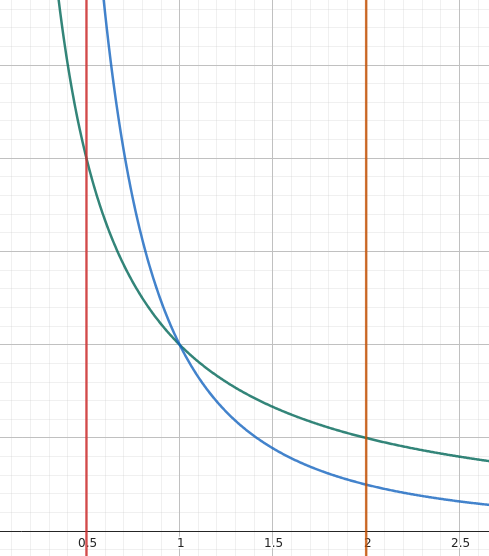
\includegraphics[width=8cm]{5D-3.2-wout.vanderborght.INF.png} \\
\end{figure}

\begin{thebibliography}{999}
%\bibitem{a} Referentie
\end{thebibliography}
\end{document} 
